\begin{frame}
  
  \frametitle {Graph partitionning}
  \begin{description}
  \item [INPUT:] \hfill \\
    \begin{enumerate}
    \item $G = (V, E)$ a $k$-connex graph 
      \begin{figure}[H]
	\begin{center}
           \scalebox{.7}{
	  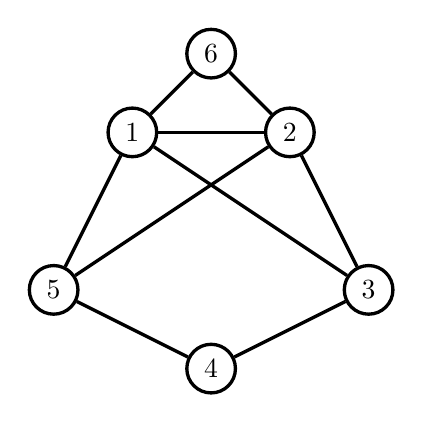
\begin{tikzpicture}
  \node[draw,circle, very thick] (A) at (1,3) {1};
  \node[draw,circle, very thick] (B) at (3,3) {2};
  \node[draw,circle, very thick] (C) at (4,1) {3};
  \node[draw,circle, very thick] (D) at (2,0) {4};
  \node[draw,circle, very thick] (E) at (0,1) {5};
  \node[draw,circle, very thick] (F) at (2,4) {6};
  \draw[very thick] (A) -- (B);
  \draw[very thick] (B) -- (C);
  \draw[very thick] (C) -- (D);
  \draw[very thick] (D) -- (E);
  \draw[very thick] (A) -- (C);
  \draw[very thick] (B) -- (E);
  \draw[very thick] (A) -- (F);
  \draw[very thick] (A) -- (E);
  \draw[very thick] (B) -- (F);

\end{tikzpicture}

}
	\end{center}
	\caption{An example of an input 3-connected graph with 6 edges}
      \end{figure}
    \item $k$
    \item $a_1, a_2 \ldots a_k$ : different vertices of $G$
    \item $n_1, n_2 \ldots n_k$ : strictly positive integers of $\sum_i n_i =  |V|$
    \end{enumerate}
    
  \end{description}
\end{frame}
\begin{frame}{Used structures and notations}
\begin{description}
\item[Partition trees] they represent a tree spanning over a partition of the graph $T_i  a_i$ being 
  the root of the partition. In this part of the presentation a tree will refer to a partition tree.
   \begin{figure}[H]
	\begin{center}
	   \scalebox{.7}{
	  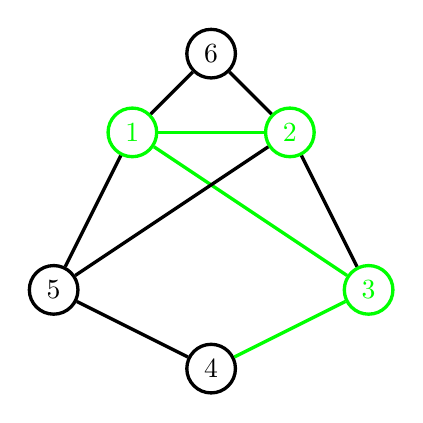
\begin{tikzpicture}
  \node[draw,circle, very thick, color=green] (A) at (1,3) {1};
  \node[draw,circle, very thick, color=green] (B) at (3,3) {2};
  \node[draw,circle, very thick, color=green] (C) at (4,1) {3};
  \node[draw,circle, very thick] (D) at (2,0) {4};
  \node[draw,circle, very thick] (E) at (0,1) {5};
  \node[draw,circle, very thick] (F) at (2,4) {6};
  \draw[very thick, color=green] (A) -- (B);
  \draw[very thick] (B) -- (C);
  \draw[very thick, color=green] (C) -- (D);
  \draw[very thick] (D) -- (E);
  \draw[very thick, color=green] (A) -- (C);
  \draw[very thick] (B) -- (E);
  \draw[very thick] (A) -- (F);
  \draw[very thick] (A) -- (E);
  \draw[very thick] (B) -- (F);

\end{tikzpicture}


	\end{center}
	\caption{An example of a partition on the input graph}
      \end{figure}
\item [Tree-Nodes] array of set of root vertices $\{a_1 \ldots a_k\}$. If $a_j \in$ Tree-node[$v$],the vertex $v$ 
  is or has been a vertex of $T_j$.
\begin{center}
  \begin{tabular}{ | l | c | r | }
    \hline                       
    Vertex & 1 & 2 & 3 & 4 & 5 \\
    \hline
    Set of roots & $\{a_1, a_2\}$ & $\{a_2\}$ & $\{a_3\}$ & \emptyset & \emptyset \\
    \hline  
  \end{tabular}
\end{center}
\item [p] The p-value of a vertex $v$ in a tree $T_i$ the ratio $\dfrac{n_i}{|T_i|}$. It ensures that the trees are properly filled during the execution of the algorithm

\end{description}
\end{frame}

\begin{frame}
             \begin{description}
                \item[OUTPUT:] \hfill \\
                        A k-partition $Par$ of G such that $\forall i \ in 1..k$ 
                        \begin{itemize} 
                                \item $H_i$ is a connected subgraph of $G$
                                \item $H_i \in Par, |V(H_i)| = n_i $
                                \item $a_i \in H_i $
                                \item $\forall j \in 1..k H_i \bigcap H_j = \emptyset$
                        \end{itemize}
        \end{description}
             \begin{figure}[H]
	       \begin{center}
	          \scalebox{.7}{
	  
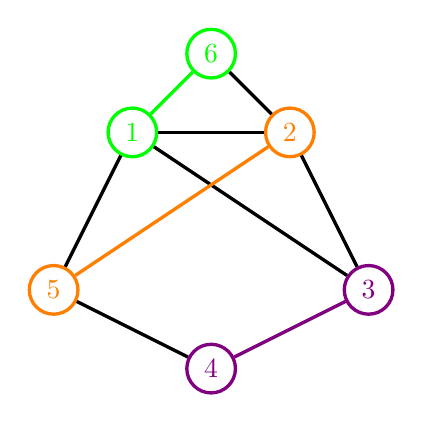
\begin{tikzpicture}
  \node[draw,circle, very thick, color=green] (A) at (1,3) {1};
  \node[draw,circle, very thick, color=orange] (B) at (3,3) {2};
  \node[draw,circle, very thick, color=violet] (C) at (4,1) {3};
  \node[draw,circle, very thick, color=violet] (D) at (2,0) {4};
  \node[draw,circle, very thick, color=orange] (E) at (0,1) {5};
  \node[draw,circle, very thick, color=green] (F) at (2,4) {6};
  \draw[very thick] (A) -- (B);
  \draw[very thick] (B) -- (C);
  \draw[very thick, color=violet] (C) -- (D);
  \draw[very thick] (D) -- (E);
  \draw[very thick] (A) -- (C);
  \draw[very thick, color=orange] (B) -- (E);
  \draw[very thick, color=green] (A) -- (F);
\draw[very thick] (A) -- (E);
  \draw[very thick] (B) -- (F);

\end{tikzpicture}


	       \end{center}
	       \caption{An example output of the 3-connected graph partition}
             \end{figure}
\end{frame}
